%!TEX root = main.tex
\section{Modelling}
This report seeks to model the infection as a function of time of a global virus outbreak. To do, firstly it will be described how one might model a virus outbreak in small uniform population. Secondly, this model will be expanded to include multiple population groups and their interactions.

\subsection{The SIR Model}
\subsubsection{Assumption}
The Susceptible-Infected-Removed model is a compartmental model assuming that within some subdivision of the population containing $N$ individuals, virus infection, cure and spread rates are i.i.d. for the 3 ``compartments'' of individuals:
\begin{itemize}
	\item Susceptible to the virus
	\item Infected by the virus
	\item Recovered and immune to the virus (or alternatively dead)
\end{itemize} 
. In reality economic status, job type, air-conditioning etc. will affect how a virus spread \cite{zika-modelling}, however, depending on the heterogeneity of the population these assumptions constitute a good approximation.

\subsubsection{Governing equations}
The SIR model is governed by 3 differential equations,
\begin{align}
\frac{d S(t)}{dt} &= - \frac{\beta}{N} I(t) S(t)   \label{eq-S}\\
\frac{d I(t)}{dt} &= \frac{\beta}{N} I(t) S(t) - \gamma I(t)  \label{eq-I}\\
\frac{d R(t)}{dt} &= \gamma I(t) \label{eq-R}
\end{align}
where $S(t), I(t)$ and $R(t)$ are functions describing the number of susceptible, infected and removed individuals at time t, $\beta$ is the rate of infection, $\gamma$ the rate of removal (dead or cured) and $N$ the total number of individuals.

From equation \eqref{eq-S} and \eqref{eq-I} one can see that susceptible individuals become infected by some ratio $\beta$ and the ratio of already infected individuals. From \eqref{eq-I} and \eqref{eq-R} one can see that infected individuals recover with a constant factor $\gamma$. 

\begin{figure}[H]
	\centering
	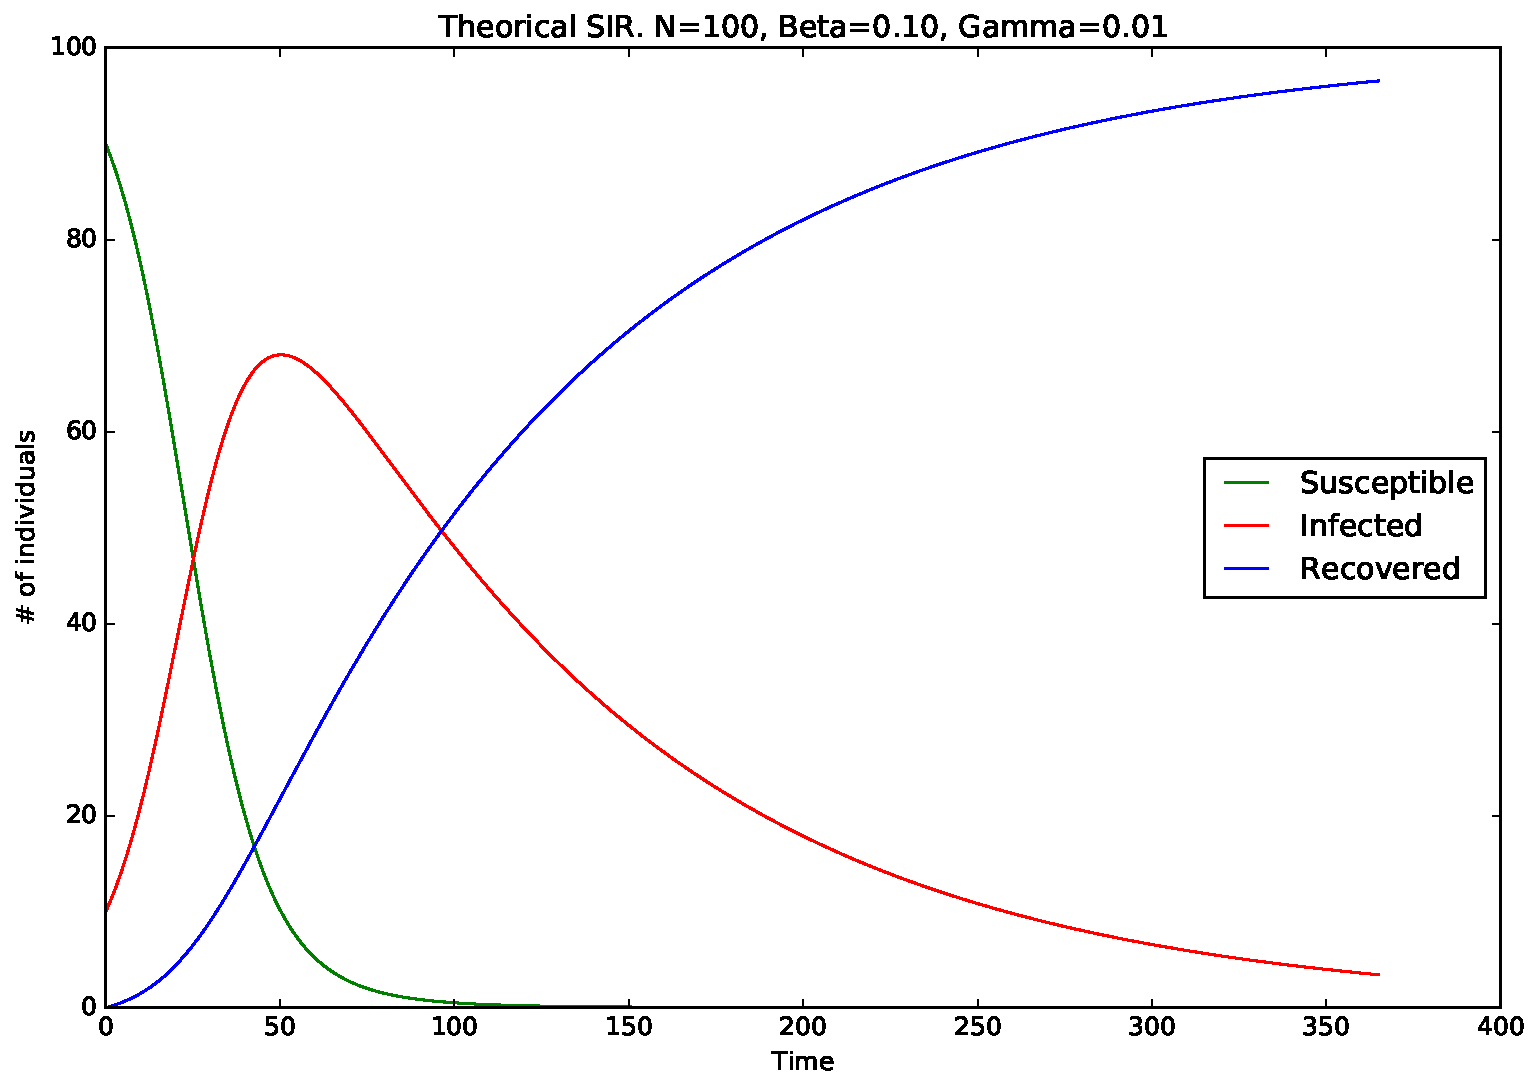
\includegraphics[width= 1.0 \linewidth]{plots/sir_one_region.pdf}
	\caption{Numerical solution to the nonlinear ODE system defining the SIR model.}
\end{figure}
\todo{comment on shape/interpretation of curve}

\subsection{Multi-region SIR}
Let it now be given that instead of having a single population, one has $K$ populations each with initial $N_k(0), S_k(0), I_k(0)$ and $R_k(0)$. Each of these populations have a probability of transferring individuals to other populations regardless of whether the individual is susceptible, infected or recovered. The governing equations are modified to add the transfers and become
\begin{align}
\frac{d S_k(t)}{dt} &= - \frac{\beta}{N_k} I(t) S(t) + \sum_{i\in K} \left( S_i(t)\tau_{i,k} - S_k(t)\tau_{k, i}\right)   &\forall k\\
\frac{d I_k(t)}{dt} &= \frac{\beta}{N_k} I(t) S(t) - \gamma I(t) + \sum_{i\in K} \left( I_i(t)\tau_{i,k} - I_k(t)\tau_{k, i}\right)  &\forall k\\
\frac{d R_k(t)}{dt} &= \gamma I(t) + \sum_{i\in K} \left( R_i(t)\tau_{i,k} - R_k(t)\tau_{k, i}\right) &\forall k
\end{align}
, where $\tau_{i,j}$ is the infinitesimal probability of transferring from population $i$ to $j$ per individual.

As an example of the above system let $K=3$ and the non zero transfer probabilities be defined by the graph:
\begin{figure}[H]
	\centering
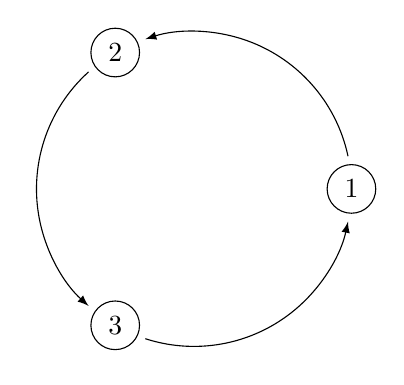
\begin{tikzpicture}

\def \n {3}
\def \radius {2cm}
\def \margin {12} % margin in angles, depends on the radius

\foreach \s in {1,...,\n}
{
	\node[draw, circle] at ({360/\n * (\s - 1)}:\radius) {$\s$};
	\draw[->, >=latex] ({360/\n * (\s - 1)+\margin}:\radius) 
	arc ({360/\n * (\s - 1)+\margin}:{360/\n * (\s)-\margin}:\radius);
}
\end{tikzpicture}
\end{figure}
. Solving this system numerically with the outbreak starting in region 1 one gets the following curves:
\begin{figure}[H]
	\centering
	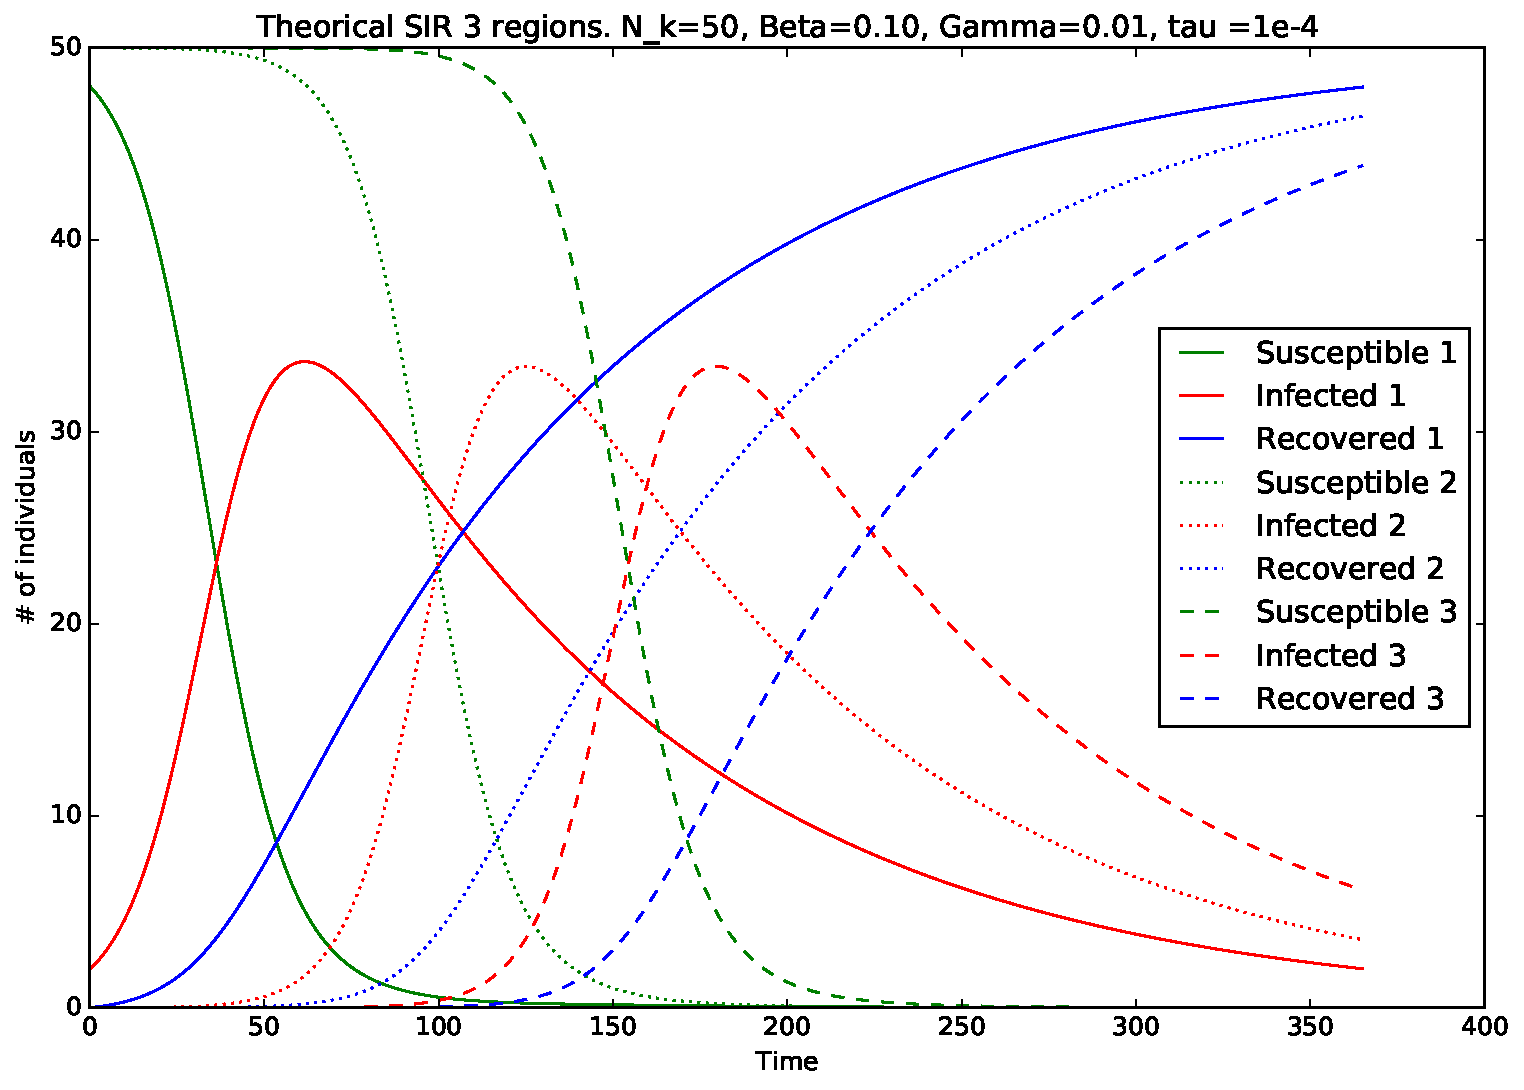
\includegraphics[width= 1.0 \linewidth]{plots/sir_three_region.pdf}
	\caption{Numerical solution to the nonlinear ODE system defining a 3-region SIR model.}
\end{figure}

From the above plot it's seen that the virus first spreads in region 1. After a certain time a enough infected individuals have been transferred to region 2 where the infection then accelerates. This continues to region 3.

\subsection{}

\subsection{Stocastic Model}

To simulate the multi-region SIR model stochastically, a binomial distribution is used to sample how many people get infected, removed and transferred. The binomial probability is chosen such the expectation is the same, as in the differential equation model.
\begin{equation*}
\begin{aligned}
\Delta I_{k,t} &= \textsc{Binom}\left(S_{k,t}, \beta \frac{I_{k, t}}{N_k}\right) \\
\Delta R_{k,t} &= \textsc{Binom}\left(I_{k,t}, \gamma\right) \\
S_{k,t} &= S_{k,t-1} - \Delta I_{k,t} + \sum_{i \in K} \left(\textsc{Binom}(S_{i,t-1}, \tau_{i,k}) - \textsc{Binom}(S_{k,t-1}, \tau_{k,i})\right) \\
I_{k,t} &= I_{k,t-1} + \Delta I_{k,t} - \Delta R_{k, t} + \sum_{i \in K} \left(\textsc{Binom}(I_{i,t-1}, \tau_{i,k}) - \textsc{Binom}(I_{k,t-1}, \tau_{k,i})\right) \\
R_{k,t} &= R_{k,t-1} + \Delta R_{k, t} + \sum_{i \in K} \left(\textsc{Binom}(R_{i,t-1}, \tau_{i,k}) - \textsc{Binom}(R_{k,t-1}, \tau_{k,i})\right)
\end{aligned}
\end{equation*}

where $\tau_{i,j}$ now is the discretized transfer probability.

\subsubsection{Transfer using Dirichlet distribution}
A problem with this approach, is the small risk that $\textsc{Binom}(S_{i, t-1}, \tau_{i,k}) = 0$ and $\textsc{Binom}(S_{k, t-1}, \tau_{k,i}) = S_k$ or similar unfortunate combination which will cause $S_{k,t}$ to become negative. This turns out to be a practical problem, to avoid this problem one should sample all the transfers for a region simultaneously such $\sum_{i \in K} \textsc{Binom}(S_{k,t-1}, \tau_{k,i}) \le S_{k, t}$.

As there does not exist a multivariate version of the binomial distribution, the Dirichlet distribution is used as an approximation. This is convenient because $\sum_{i} X_{i,k} = 1$ if $\mathbf{X}_k \sim \textsc{Dir}(\boldsymbol{\alpha}_k)$. Because the Dirichlet distribution has support $X_i \in [0, 1]$, $\floor*{N_k X_{i,k}}$ is used.

Furthermore to reduced the amount of sampling, the total transfer $T$ is sampled instead of sampling $S$, $I$ and $R$ independently.

To approximate the binomial distribution using a Dirichlet distribution the expectation is set to be the same. To simplify notation region $k$ is omitted from the subscript and the summarization of $tau_k$ and $\alpha_i$ is introduced:
\begin{equation}
\tau_s = \sum_{k = 1}^{K} \tau_k, \quad \alpha_s = \sum_{k = 1}^{K+1} \tau_k
\end{equation}

\begin{equation}
\mathbb{E}[T_{i}] = \mathbb{E}[N X_i] \Leftrightarrow N \tau_i = N \frac{\alpha_i}{\alpha_s} \quad \forall i \in K
\label{dir-expected-trans}
\end{equation}

To allow $\sum_{i} X_{i,k} \le 1$ the Dirichlet distribution is extended with another variable $X_{k, K+1}$, which will be how large a proportion region $k$ should keep.
\begin{equation}
\mathbb{E}[T_{K+1}] = \mathbb{E}[N X_{K+1}] \Leftrightarrow N \left(1 - \tau_s\right) = N \frac{\alpha_{K+1}}{\alpha_s}
\label{dir-expected-stay}
\end{equation}
  
This is a linear system with n variables and n equations, but it turns out not to have full rank. To add another equation the variance of $T_{K+1}$ is also set to be the same.
\begin{equation}
\textsc{Var}[T_{K+1}] = \textsc{Var}[N X_{K+1}] \Leftrightarrow N\tau_s (1 - \tau_s) = N^2 \frac{\alpha_{K+1}(\alpha_s - \alpha_{K+1})}{\alpha_s^2 (\alpha_s + 1)}
\label{dir-var}
\end{equation}

The trick to solving this set of equations, is to isolate $\alpha_s$ from \eqref{dir-expected-stay} and insert it into \eqref{dir-expected-trans} and \eqref{dir-var}.
\begin{align}
\alpha_s &= \frac{\alpha_{K+1}}{1 - \tau_s} \label{dir-expected-intermediate} \\
N \tau_i &= N \frac{\alpha_i}{\frac{\alpha_{K+1}}{1 - \tau_s}} \quad \forall i \in K \\
N\tau_s (1 - \tau_s) &= N^2 \frac{\alpha_{K+1}\left(\frac{\alpha_{K+1}}{1 - \tau_s} - \alpha_{K+1}\right)}{\left(\frac{\alpha_{K+1}}{1 - \tau_s}\right)^2 \left(\frac{\alpha_{K+1}}{1 - \tau_s} + 1\right)} \label{dir-var-intermediate}
\end{align}

$\alpha_{K+1}$ can now be isolated from \eqref{dir-var-intermediate} yielding
\begin{equation}
\alpha_{K+1} = (N - 1) - \tau_s (N - 1)
\end{equation}
, inserting this into \eqref{dir-expected-intermediate} gives:
\begin{equation}
\alpha_{i} = \tau_i (N - 1)
\end{equation}
Using the $\alpha_{i}$ solution $\alpha_{K+1}$ can now be reformulated as
\begin{equation}
\alpha_{K+1} = (N - 1) - \sum_{i=1}^K \alpha_k
\end{equation}
which is computationally slightly more convenient.

\begin{figure}[H]
	\centering
	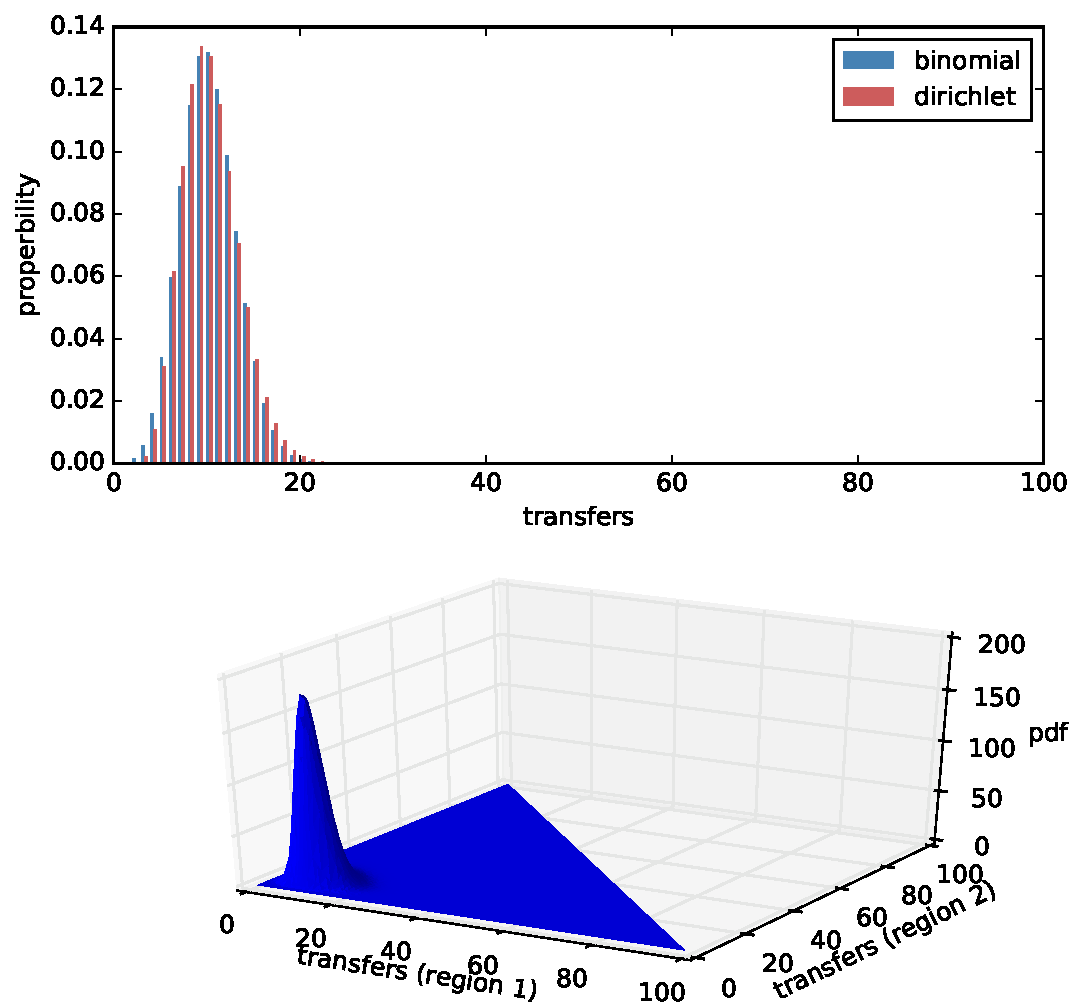
\includegraphics[width= 1.0 \linewidth]{plots/dirichlet-validation}
	\caption{A dirichlet distribution  upscaled by $N$, with $\tau = (0.1, 0.1)$ and $N = 100$. First figure compare the marginal probability $P(\floor*{N X_1})$ with the binomial distribution. Second figure shows the Dirichlet pdf with $X_3 = 1- X_1 - X_2$.}
\end{figure}


